%!TEX root = ../presentation.tex

\section{Security Models}

\begin{frame}
  \frametitle{Bell-LaPadula}
  \begin{columns}
    \begin{column}{.5\textwidth}
      \begin{itemize}
        \item Authorization
        \item No read-up
        \item No write-down
      \end{itemize}
      \vspace{5em}
    \end{column}
    \begin{column}{.5\textwidth}
      \centering
      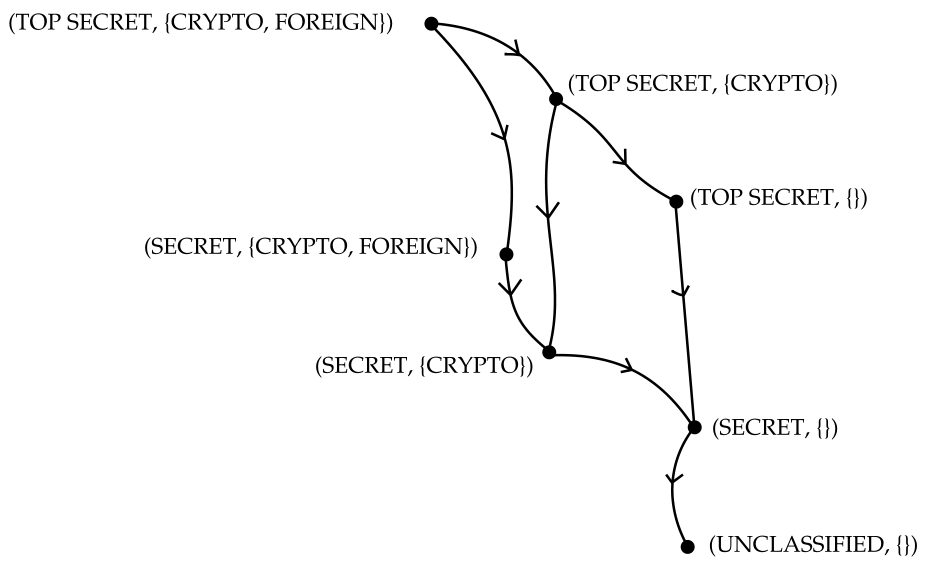
\includegraphics[height=.7\textheight]{graphics/blp_lattice}
    \end{column}
  \end{columns}
\end{frame}

\begin{frame}
  \frametitle{Chinese Wall}

  \begin{itemize}
    \item Conflict of interest
    \item Similar properties to Bell-LaPadula
  \end{itemize}
  \vfill
  \begin{columns}
    \begin{column}{.33\textwidth}
      \includegraphics[height=.3\textheight]{graphics/chineseSituation}
    \end{column}
    \begin{column}{.33\textwidth}
      \includegraphics[height=.3\textheight]{graphics/chineseChoice1}
    \end{column}
    \begin{column}{.33\textwidth}
      \includegraphics[height=.3\textheight]{graphics/chineseChoice2}
    \end{column}
  \end{columns}
\end{frame}

\begin{frame}
  \frametitle{Decentralized Label Model}

  \begin{itemize}
    \item Controlling information flow
    \item Decentralized
  \end{itemize}

  \vfill

  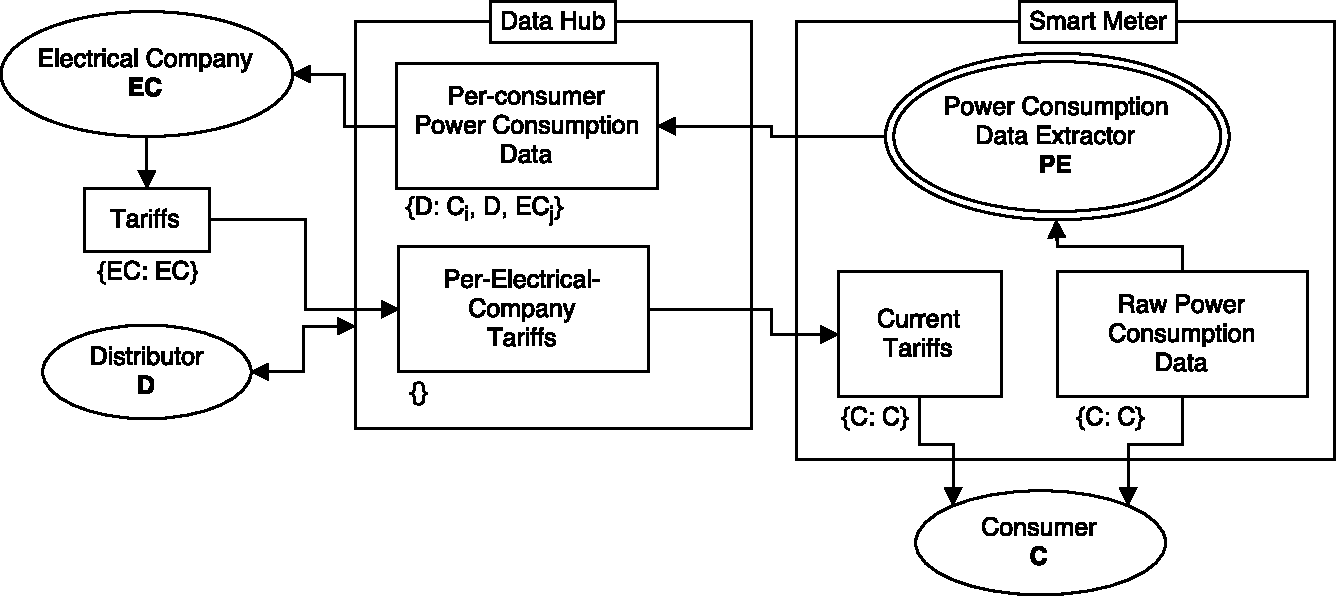
\includegraphics[width=\textwidth]{graphics/dlm_sm_example}
\end{frame}
